% Template for PLoS
% Version 3.4 January 2017
\documentclass[10pt,letterpaper]{article}
\usepackage[top=0.85in,left=2.75in,footskip=0.75in]{geometry}

% amsmath and amssymb packages, useful for mathematical formulas and symbols
\usepackage{amsmath,amssymb}

% Use adjustwidth environment to exceed column width (see example table in text)
\usepackage{changepage}

% Use Unicode characters when possible
\usepackage[utf8x]{inputenc}

% textcomp package and marvosym package for additional characters
\usepackage{textcomp,marvosym}

% cite package, to clean up citations in the main text. Do not remove.
% \usepackage{cite}

% Use nameref to cite supporting information files (see Supporting Information section for more info)
\usepackage{nameref,hyperref}

% line numbers
\usepackage[right]{lineno}

% ligatures disabled
\usepackage{microtype}
\DisableLigatures[f]{encoding = *, family = * }

% color can be used to apply background shading to table cells only
\usepackage[table]{xcolor}

% array package and thick rules for tables
\usepackage{array}

% create "+" rule type for thick vertical lines
\newcolumntype{+}{!{\vrule width 2pt}}

% create \thickcline for thick horizontal lines of variable length
\newlength\savedwidth
\newcommand\thickcline[1]{%
  \noalign{\global\savedwidth\arrayrulewidth\global\arrayrulewidth 2pt}%
  \cline{#1}%
  \noalign{\vskip\arrayrulewidth}%
  \noalign{\global\arrayrulewidth\savedwidth}%
}

% \thickhline command for thick horizontal lines that span the table
\newcommand\thickhline{\noalign{\global\savedwidth\arrayrulewidth\global\arrayrulewidth 2pt}%
\hline
\noalign{\global\arrayrulewidth\savedwidth}}


% Remove comment for double spacing
%\usepackage{setspace} 
%\doublespacing

% Text layout
\raggedright
\setlength{\parindent}{0.5cm}
\textwidth 5.25in 
\textheight 8.75in

% Bold the 'Figure #' in the caption and separate it from the title/caption with a period
% Captions will be left justified
\usepackage[aboveskip=1pt,labelfont=bf,labelsep=period,justification=raggedright,singlelinecheck=off]{caption}
\renewcommand{\figurename}{Fig}

% Use the PLoS provided BiBTeX style
% \bibliographystyle{plos2015}

% Remove brackets from numbering in List of References
\makeatletter
\renewcommand{\@biblabel}[1]{\quad#1.}
\makeatother

% Leave date blank
\date{}

% Header and Footer with logo
\usepackage{lastpage,fancyhdr,graphicx}
\usepackage{epstopdf}
\pagestyle{myheadings}
\pagestyle{fancy}
\fancyhf{}
\setlength{\headheight}{27.023pt}
\lhead{
\includegraphics[width=2.0in]{PLOS-submission.eps}}
\rfoot{\thepage/\pageref{LastPage}}
\renewcommand{\footrule}{\hrule height 2pt \vspace{2mm}}
\fancyheadoffset[L]{2.25in}
\fancyfootoffset[L]{2.25in}
\lfoot{\sf PLOS}

%% Include all macros below
\newcommand{\lorem}{{\bf LOREM}}
\newcommand{\ipsum}{{\bf IPSUM}}





\usepackage{forarray}
\usepackage{xstring}
\newcommand{\getIndex}[2]{
  \ForEach{,}{\IfEq{#1}{\thislevelitem}{\number\thislevelcount\ExitForEach}{}}{#2}
}

\setcounter{secnumdepth}{0}

\newcommand{\getAff}[1]{
  \getIndex{#1}{Smith College}
}

\providecommand{\tightlist}{%
  \setlength{\itemsep}{0pt}\setlength{\parskip}{0pt}}

\begin{document}
\vspace*{0.2in}

% Title must be 250 characters or less.
\begin{flushleft}
{\Large
\textbf\newline{Classifying Socially Impactful Articles} % Please use "sentence case" for title and headings (capitalize only the first word in a title (or heading), the first word in a subtitle (or subheading), and any proper nouns).
}
\newline
\\
Julianna Alvord\textsuperscript{\getAff{Smith College}},
Minji Kang\textsuperscript{\getAff{Smith College}},
Zainab Rizvi\textsuperscript{\getAff{Smith College}},
Erina Fukuda\textsuperscript{\getAff{Smith College}}\\
\bigskip
\textbf{\getAff{Smith College}}Statistical \& Data Sciences, 1 Chapin Way Northampton, Massachusetts
01063\\
\bigskip
\end{flushleft}
% Please keep the abstract below 300 words
\section*{Abstract}
Our aim is to create a metric to measure how socially impactful an
article is. We used articles from the politics section of a major online
news publishing house for this purpose. We define an article to be
socially impactful if the topic being discussed is important, if it can
change the way readers think, reaffirm their thinking, or leave an
impression on them. For our classifier, we used a dataset that contained
social media statistics and traffic information for each article (such
as page views, Facebook comments etc.), some basic NLP statistics for
the text of the article, and sentiment analysis of the text. We manually
classified the articles as 0 if they are not socially impactful and 1 if
they are. We then trained three models (Gradient Boosting Model, Support
Vector Machines, and Logistic Regression) and predicted probabilities
for each article. We present our results in a Shiny application with a
user-friendly interface that displays the results of our models. The
application also provides information on the important predictors for
each model and the overall distribution of probabilities. Through this
information, users are able to decide for themselves the best model
score to use for a particular article.

% Please keep the Author Summary between 150 and 200 words
% Use first person. PLOS ONE authors please skip this step. 
% Author Summary not valid for PLOS ONE submissions.   

\linenumbers

% Use "Eq" instead of "Equation" for equation citations.
\hypertarget{introduction}{%
\section{Introduction}\label{introduction}}

Our team used articles from a major online news publication and tried to
create a tool that could automatically classify socially impactful
articles from those that are not based on several aspects of the
article. These aspects included the article's presence in social media
(e.g.~number of likes, shares, etc.), amount of traffic (e.g page views,
engaged minutes, etc.), level of readability and the sentiments
associated with the words used.

We define socially impactful articles as those that change the readers'
way of thinking. It can also bring someone to take action or change the
way they act. Even if it does not make them change their views, if the
article leaves an impression or makes readers think it can also be a
socially impactful article as well. Therefore, some impacts that the
article can have on readers are changing the way they think, leaving an
impression, or reaffirming their ideas. It could also make readers
change their habits or actions based on what they have read. These
definitions were condensed into a flowchart that was used for future
classification (See Figure 1).

Figure 1: social impact definition flow chart{]}(tree.png)

\#\#\#Importance of Social Impact

This project will allow for the news publication to

\hypertarget{pre-existing-data}{%
\paragraph{Pre-existing Data}\label{pre-existing-data}}

The data for this project were provided by the online news source which
contained information for their top 10000 most-viewed articles. This
news source collects and calculates data on many variables such as page
views, returning visitors, and social interactions for each of their
articles. The dataset given to us included 33 variables, the majority of
which were numeric. To understand these metrics, we referred to the
company's application programming interface (API) which contained a
description of 21 metrics. The API can be found at this address:
\url{https://www.parse.ly/help/api/available-metrics/}.

Other numeric metrics not included in this API were average views for
returning and new visitors, as well as direct, other, internal, and
search referrals. Direct referrals are a count of \ldots{}

The final six variables(??? what do you mean by final 6) included the
URL, title, publish date, author(s), section, and tags. Example of tags
are `ads\_scary' and `health\_depression'. Some sections include
`Crime', `Comedy', `Entertainment', and `Politics'.

\hypertarget{descriptive-statistics}{%
\paragraph{Descriptive Statistics}\label{descriptive-statistics}}

For this entire dataset of 10,000 observations, the average numbers of
page views was 105904.9. The average number of social interactions was
12957.97. An average of 77584.06 engaged minutes were spent on each
article. The top three sections were Politics (27.94\% of articles),
Entertainment (18.62 \%), and Comedy (4.86\%).

\hypertarget{subsetting-our-data}{%
\paragraph{Subsetting our Data}\label{subsetting-our-data}}

While initially defining social impact, we discovered the difficulty of
comparing articles from different sections. For example, an article from
the entertainment section would never seem socially impactful when
compared to an article from a section like ``Black Voices.''

Existing literature also indicates that text mining models perform
better when they are domain-specific and that it is difficult to compare
results across different domains.

We decided that this project needed to start with only one section. The
section chosen was politics because it had the highest number of
articles which was 2,794.

\hypertarget{data}{%
\section{Data}\label{data}}

\hypertarget{collection-of-additional-data}{%
\subsubsection{Collection of Additional
Data}\label{collection-of-additional-data}}

\hypertarget{text-mining}{%
\paragraph{Text Mining}\label{text-mining}}

We realized that all of our existing data tell us about the the
behavioral data of each article (i.e what the reader is actively doing
with each article). However, one of the problems specified by our client
was that behavioral analysis is oftentimes not a good indicator of
whether the article is socially impactful or not. This is because it
fails to take the actual content of the articles into account. Thus in
order to add another dimension to our data, we decided to retrieve the
text of the articles from the URLs that were provided to us in the
dataset.

We wrote a Python script that takes in the URL as input and scrapes the
webpage to retrieve the text. We used the \texttt{BeautifulSoup} package
in Python for this purpose {[}1{]}.

\emph{Incorporating Natural Language Processing Statistics} We decided
to supplement the social media statistics we got from our client with
some basic text mining statistics that give us some information about
the text. As discussed earlier, since the task at hand is to judge the
impact of the articles, we made the assumption that there would be some
relationship between the text itself and the impact it creates.

We wrote a script in Python for this purpose using the \texttt{textstat}
Python package {[}2{]}.The script takes as input the text of the
articles (obtained from the parser) and outputs the computed statistics.
Specifically, we calculate the following five statistics:

\begin{enumerate}
\def\labelenumi{\arabic{enumi}.}
\tightlist
\item
  word\_count: This calculates the number of words in the text.
\item
  sentence\_count: This calculates the number of sentences in the text.
\item
  readability\_score: This calculates the Flesch Reading Ease Score
  which is helpful to access the ease of readability in a document and
  ranges from 0 to 100 where 0 is difficult to read and 100 is easy to
  read {[}3{]}.
\item
  grade\_level: This is calculated using the Automated Readability Index
  which outputs a number that approximates the grade level needed to
  comprehend the given text. This ranges from 1 to 12 {[}4{]}.
\item
  smog\_index: This calculates the a statistics called Simple Measure of
  Gobbledygook for the given text. In simple terms, smog index
  calculates the difficulty level of a sentences based on the number of
  words that are polysyllabic. It ranges from 5 to 22 which corresponds
  to the age of the reader who can understand the given text {[}5{]}.
\end{enumerate}

\emph{Sentiment Analysis} We used the \texttt{tidytext} package's
\texttt{AFINN} lexicon as an effort to have an idea about what
sentiments were present in each article without manually going through
each one of them. \texttt{AFINN} consists of around 2500 words and
phrases scored between -5 to +5. The numbers reflect the severity of the
word (e.g. ``breathtaking'' seems stronger than ``relieve'' which are
positive 5 and 1 words respectively) and the signs imply the positivity
of the word.

We scraped the text of the articles, broke it up into individual words
and omitted any stop words, which are commonly used words that should be
ignored (e.g. ``the'', ``and'', ``is''). Then, the words in
\texttt{AFINN} were joined with the articles' words, and the number of
words present in the articles with a rating in \texttt{AFINN} were
totaled. By using this method, we were able to add a column for -5 to -1
and +1 to +5 and label what percent of all words existing in AFFIN
(excluding 0-rated words) fell into each category of ratings. For
example, the column, \texttt{pos1} was created by taking the number of
words rated +1 in the text and dividing it by all words with any rating
other than 0 in AFINN. Naturally, the higher in rating number
(e.g.~negative and positive 5), the fewer instances there seemed to be
which makes sense, given that those words were more extreme and
therefore more likely to choose the occasions in which they appeared in
an article.

However, this sentiment analysis has some limitations. The first is that
the text was broken up into individual words. Therefore, words that go
together such as ``not good'' (a negative 2 phrase in AFINN) are not be
accounted for because it is split up into ``not'' and ``good''. ``Not''
does not have a rating in AFINN, and ``good'' has a rating of positive
3. Thus, in that article, the positive 2 variable have an increase in
percentage even though the in reality, negative 2 should have the
increase. In addition, the system is unable to take context into
consideration. For example, if an article was referring to ``swift'' as
a name (e.g.~Taylor Swift), the sentiment analysis will not be able to
distinguish it from the adjective ``swift'' which is given a rating of
+2. Therefore, the +2 word percentage rate will increase due to the word
usage in the text, even though it should not part of the rating. Given
these two limitations, if an article was very short and did not have
many words that existed in \texttt{AFINN}, there is a possibility that
only one word had a rating attached to it. If that is the case, 100\% of
that article's sentiment is that one sentiment. If, coincidentally, the
word that matched was erroneous such as ``not good'', the addition of
the sentiment variable is actually misleading and detrimental to our
analyses.

\hypertarget{article-classification}{%
\paragraph{Article Classification}\label{article-classification}}

In order to run supervised learning models, we needed to populate the
response variable (Impact) to create the training set. Thus, we decided
to use Amazon Mechanical Turk (MTurk) for data collection to ensure the
classification of articles were random. MTurk is a crowd sourcing
internet marketplace where ``Requesters'' create tasks that require
human intelligence and ``Workers'' are paid upon successful completion
of each task also known as HITs (Human Intelligence Tasks).

As requesters, we launched tasks that provided a hyperlink to an article
and the flow chart shown in Figure 1. For each HIT the workers were
asked to click the hyperlink to be directed to the article, read the
article, and classify the articles after following the given flow chart.
We launched 2500 articles and requested 3 iterations of each article.
Thus, we had a total of 7500 HITs. Upon data collection, analysis of the
7500 HITs was conducted. We conducted a Pearson correlation test of
association between paired samples of the three iteration. The results
of the test indicated that none of the interactions were statistically
significantly correlated to one another (p-value \textgreater{} 0.05).
Due to the low correlation value of iterations, another analysis was
conducted to test whether the data was indistinguishable from random
data. We conducted a test of significant difference between two
independent correlations of random imputation of the classification of
articles to the three iterations. The results indicated that there were
no statistically significant difference between random imputation data
and the data collected through MTurk (p-value \textgreater{} 0.05).

Following the results of the first MTurk, we launched another set of
tasks that provided the parsed text of the article and same flow chart
from the previous task. For each HIT the workers were asked to read the
parsed text, summarize the text in two to five sentences, and classify
the articles after following the given flow chart. This time, we
launched 500 articles with 3 iterations of each articles. Thus, we had a
total 1500 HITs. The results of the data collection had 97\% of the
articles rated as socially impactful. The results of the secound MTurk
data was not realistic to our understanding of social impact, and would
have not been a ideal data for training set (as any classification model
will predict everything as impactful). Thus, this data was discarded as
well.

Finally, the data collection was conducted by our group members going
through each articles and classifying the articles ourselves following
the flow chart in Figure 1. We classified a total of 1300 articles and
used the 1300 articles as the training set.

\hypertarget{data-preparation}{%
\subsubsection{Data Preparation}\label{data-preparation}}

Once the NLP and sentiment analysis was completed, the original
pre-existing data, the new NLP, sentiment analysis, and the social
impact classification outcome were compiled together. In order to build
supervised learning models, only numerical vectors were selected for
data analysis. Thus variables such as \texttt{Tags},
\texttt{Published\_Date}, \texttt{Author} and the parsed \texttt{Text}
was removed. However we kept \texttt{URL} and \texttt{Title} variables,
but those were not included in the models. Additionally, six duplicated
rows were removed.

\emph{Missing Data} There were a few missing entries in the traffic data
given by our client. Not all of the articles have been shared on every
single media platform which created missing entries within our data set.
In order to account for missing data of different social references and
interaction with social media of the articles, a dummy variable was
created that indicated whether the article has been shared in each of
the different social media platforms. On the other hand, all the
articles have been shared on Facebook and Twitter. Thus two new
variables were created that counted the interaction and references on
social media platform other than Facebook and Twitter. Additionally, we
created new variables that scaled some vectors that had a large range to
be used for logistic regression's odds ratio calculation, because often
the units were too small to interpret the odds. Therefore,
\texttt{Engaged\_minutes} was divided by 60 to create
\texttt{Engaged\_hours}. In addition, \texttt{Returning\_vis},
\texttt{Search\_refs}, \texttt{Internal\_refs}, \texttt{Other\_refs},
\texttt{Direct\_refs}, \texttt{Fb\_refs}, \texttt{Tw\_refs},
\texttt{Fb\_interactions} were divided by 10000 (indicated by adding
\texttt{\_10000} after each variable), and \texttt{word\_count} was
divided by 10 to create the variable, \texttt{total\_words\_10}.

\hypertarget{mysql-database}{%
\paragraph{MySQL database}\label{mysql-database}}

Once we had the data cleaned, we uploaded it on a MySQL Server database.
Even though we are currently only working with around 2700 articles, we
wanted to make sure that our project is scalable. Putting the dataset in
a database also unified the schema for our different models.

\hypertarget{models}{%
\section{Models}\label{models}}

We used various machine learning models for our classification problem.
Our explanatory variables were the social media, NLP, and sentiment
statistics whereas our response variable was our classification of the
article as 0 or 1.

To evaluate our models, we used four criteria:

\begin{enumerate}
\def\labelenumi{\arabic{enumi}.}
\tightlist
\item
  Specificity: Correctly identified socially impactful articles or 1's
\item
  Sensitivity: Correctly identified non-socially impactful articles or
  0's
\item
  Area under Receiver Operating Curve: The probability that the
  classifier will assign a higher score to a randomly chosen positive
  example than to a randomly chosen negative example.
\item
  Accuracy: Rate of correct predictions.
\end{enumerate}

In the end, we decided to use gradient boosting trees, support vector
machines, and logistic regression.

The base line comparison for our models is the null model which has an
accuracy of 63\%. This is because we classified 37\% of the articles as
socially impactful so if a model were to guess everything as not being
socially impactful, it would be correct 63\% of the time.

\hypertarget{decision-tree}{%
\paragraph{Decision Tree}\label{decision-tree}}

Decision trees provide comprehensive analysis of each decision and
partitions the data accordingly {[}6{]}. We chose to use gradient
boosting as one of our model because it avoids over fitting and reduces
variance, unlike other decision tree models {[}6{]}. Given a baseline
model, boosting fits a decision tree to the residuals from the baseline
model {[}6{]}. Then, Boosting grows trees sequentially allowing the next
tree to be fitted into a function to update their residuals {[}6{]}.
Since boosting learns information from previous trees, the error rate is
also usually lower than other forest models {[}6{]}. Additionally,
boosting has three tuning parameters:

\begin{itemize}
\tightlist
\item
  The number of trees: total number of trees that will be grown {[}6{]}.
\item
  The shrinkage parameter: The rate at which boosting learns {[}6{]}.
\item
  Number of splits in each tree: controls the complexity of the model
  {[}6{]}.
\end{itemize}

\begin{figure}
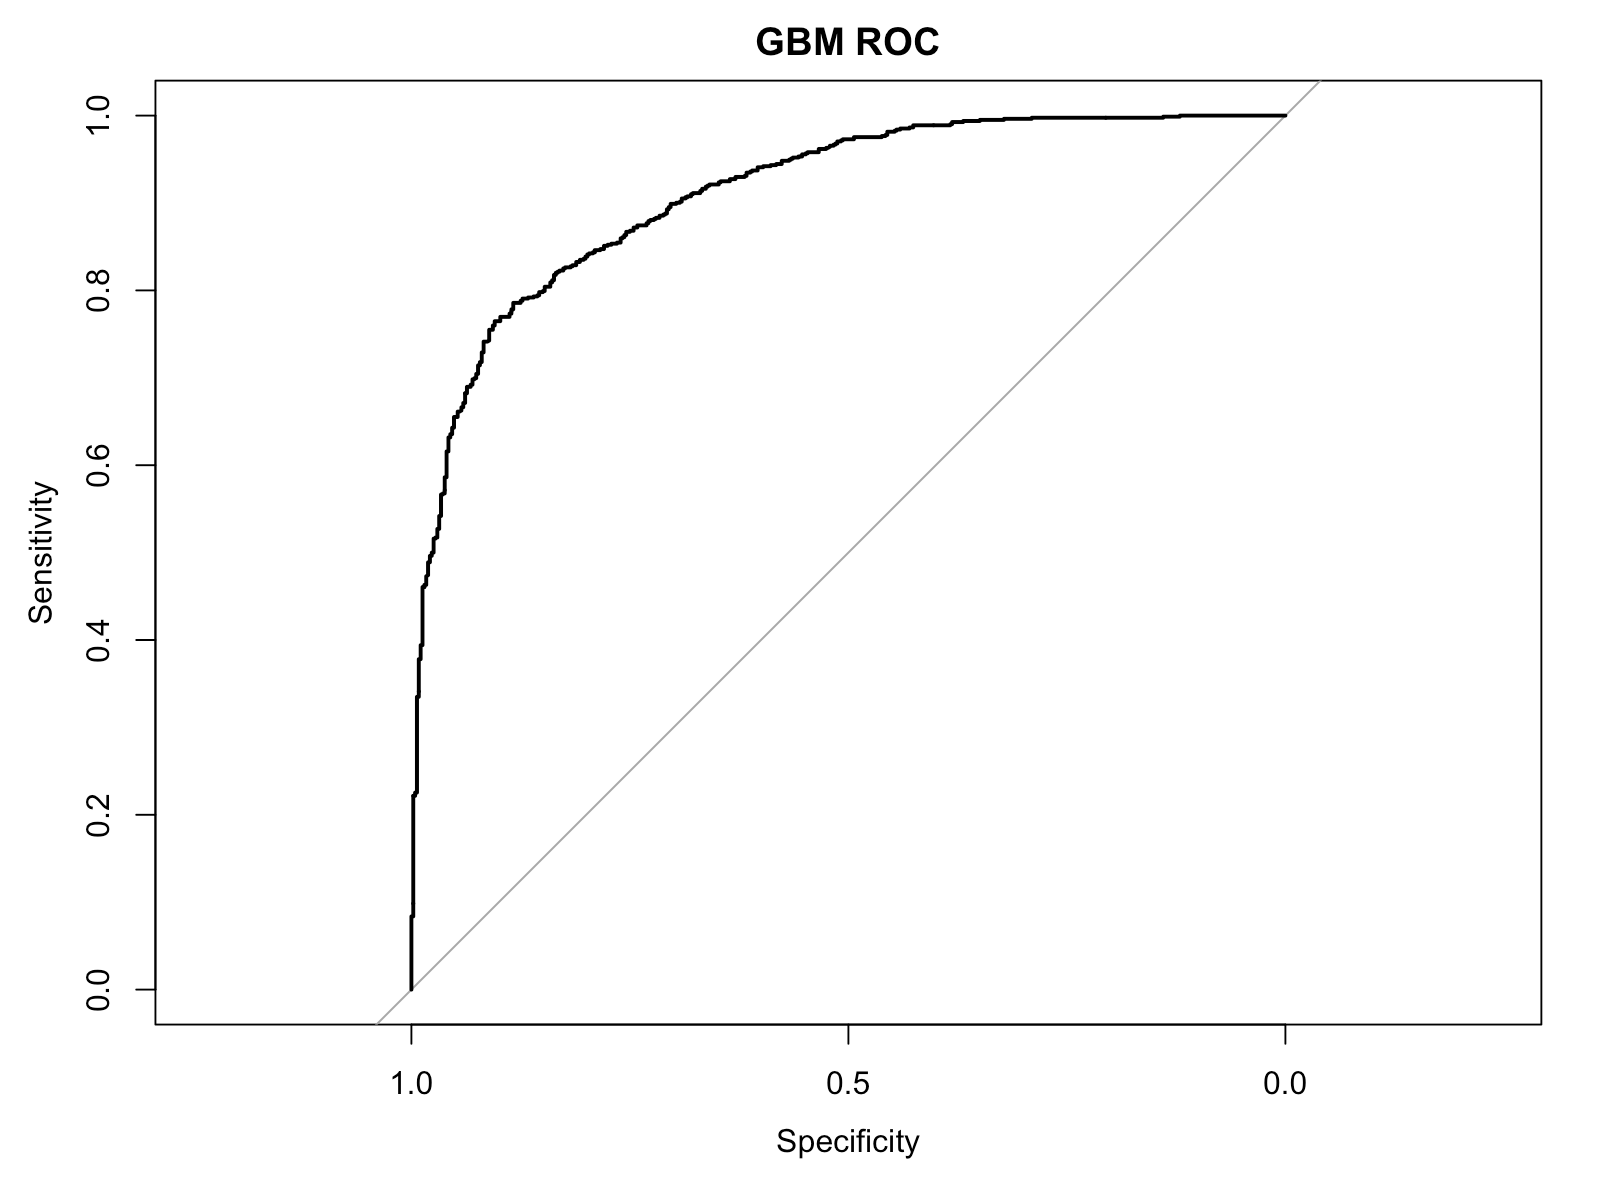
\includegraphics[width=400px,height=300px]{roc_gbm} \caption{ROC curve of Gradient Boosting model}\label{fig:unnamed-chunk-1}
\end{figure}

\begin{figure}
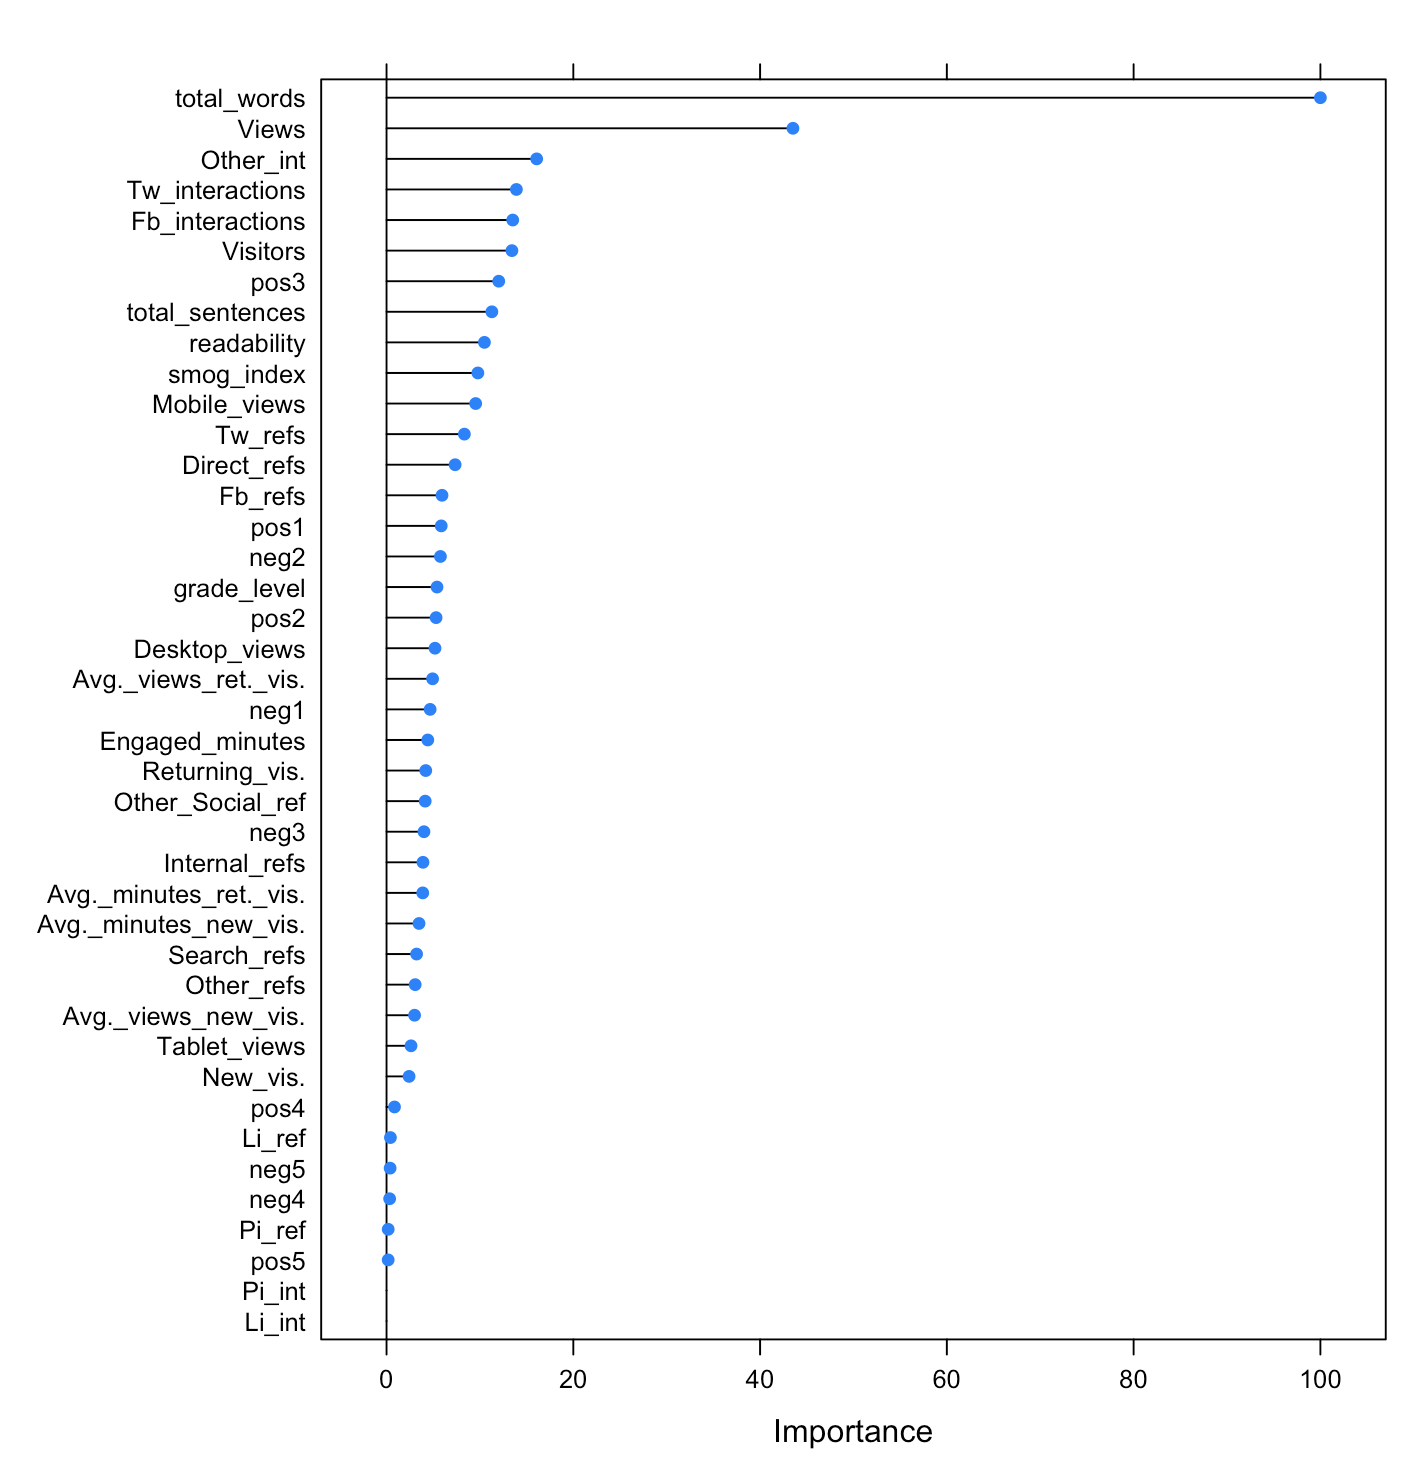
\includegraphics[width=400px,height=300px]{boost_VarImp} \caption{Variable Importance of boosting model}\label{fig:unnamed-chunk-2}
\end{figure}

\begin{figure}
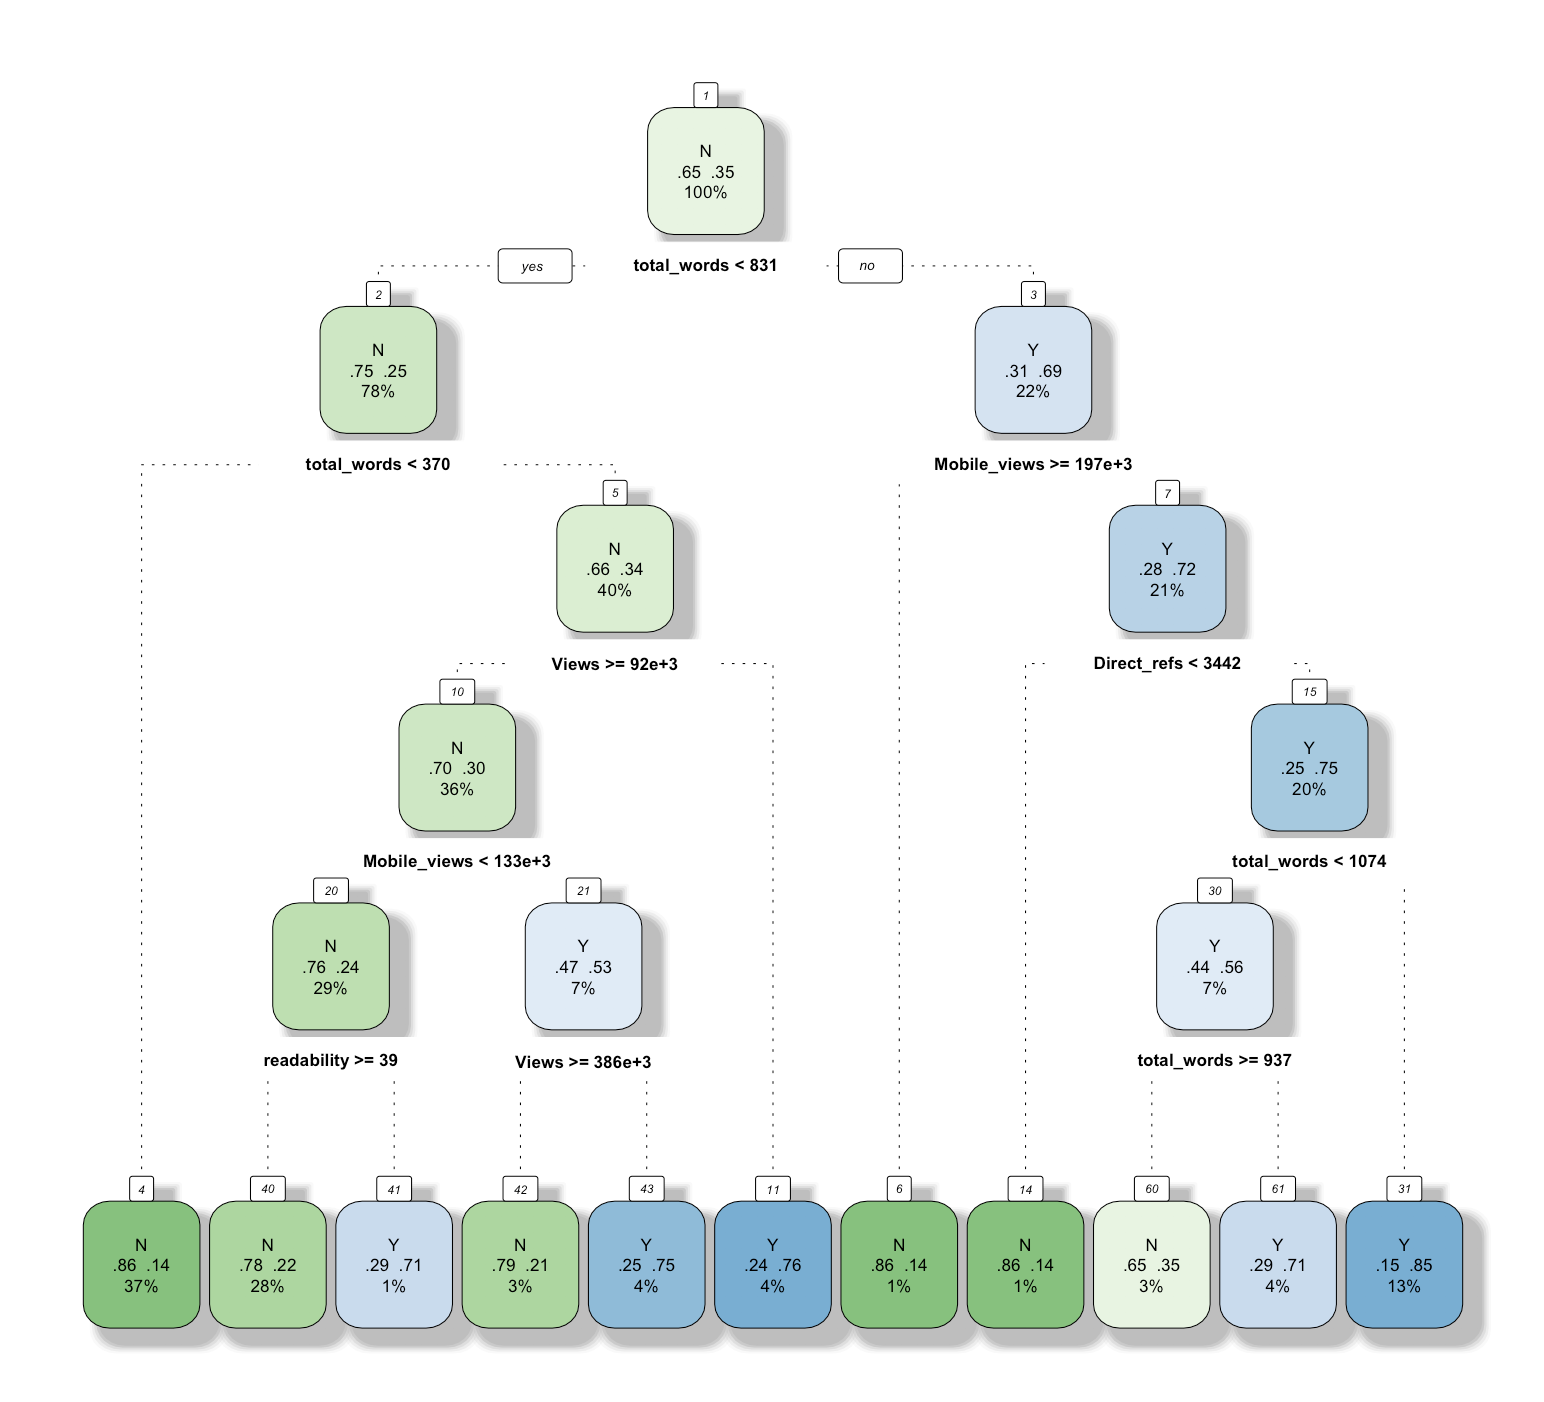
\includegraphics[width=400px,height=300px]{classification-Tree} \caption{ Classification tree using top 20 variables selected from GBM}\label{fig:unnamed-chunk-3}
\end{figure}

Using the \texttt{caret} package in R {[}7{]}, the gradient boosting
model split the data internally and ran its own training and testing
models with five cross validation folds. The model also tuned the
parameter with five cross validation folds. The optimal tuning
parameters with the highest Receiver Operating Characteristics (ROC =
0.792) was 900 trees with shrinkage of 0.01, number of splits of 3. The
\texttt{gbm} in the caret package offers another parameter that measures
the minimum number of observations in tree's terminal nodes. The optimal
tuning parameter for the minimum number of observation in the terminal
node was 8. Thus, these parameters were used for the final model. The
gradient boosting model had an accuracy of 82.5\% and the 95\%
confidence interval for accuracy was between 80\% and 84.5\%. In
addition the model also showed high sensitivity value of 0.901, but a
lower specificity value of 0.609. The ROC curve is shown in Figure 2.
Thus the model was positively classifying impactful articles better than
negatively classifying impactful articles (AUROC = 0.911). The top 25
most important variables of the boosting model results are shown in
Figure 3.

Lastly, we created a classification tree using the top 20 variables
selected from the boosting tree using \texttt{rpart} package in R
{[}8{]}, shown in figure 2.

\hypertarget{support-vector-machines}{%
\paragraph{Support Vector Machines}\label{support-vector-machines}}

An SVM is a vector space-based classification machine learning method
where the goal is to find a decision boundary between two classes that
is maximally far from any point in the training data (possibly
discounting some points as outliers or noise){[}6{]}.

Our main motivation for using Support Vector Machines to classify the
articles was that SVMs are known to perform well in text classification
tasks, especially with small training sets. We use the \texttt{e1071}
package in R and trained the SVM on our entire set of 1284 classified
articles {[}9{]}.

\begin{figure}

\includegraphics[width=400px,height=300px]{roc-curve} \caption{ROC Curve for SVM model}\label{fig:unnamed-chunk-4}
\end{figure}

A kernel is a compact representation of the similarity in the dataset.
Since we are working with multidimensional data, we tried linear,
polynomial, sigmoid and radial kernels to see which one gave us the
highest accuracy. After cross-validation and tuning, we found that a
radial kernel performs best on our data with a low cost and high gamma
value.

We found the accuracy of our model to be 79.44\%. The sensitivity is
0.92 and the specificity is 0.56. The AUROC value is 0.87. The ROC curve
of the result is show in figure 5.

\hypertarget{logistic-regression.-to-be-changed-due-to-changes-in-data-variablesmodel}{%
\paragraph{Logistic Regression. (to be changed due to changes in data +
variables/model)}\label{logistic-regression.-to-be-changed-due-to-changes-in-data-variablesmodel}}

We fit a step-wise logistic regression as another way to determine
whether an article had social impact. We optimized for AIC and found
that \texttt{Average\ views\ by\ returning\ visitors},
\texttt{smog-index}, \texttt{Sentiments} (i.e. \texttt{neg1},
\texttt{neg2}, \texttt{neg3}, \texttt{neg4}, \texttt{pos1},
\texttt{pos2} and \texttt{pos4}),
\texttt{LinkedIn\ \&\ other\ referrals}, \texttt{Facebook\ interactions}
and \texttt{Length} all had positive coefficients. In other words, a one
unit increase in these variables increased the probability that an
article would be socially impactful. However, interestingly,
\texttt{Mobile\ views} and \texttt{Engaged\ Hours} had negative impact.
We cannot say for certain why this may be the case. We suspected that it
could be due to certain human behaviors linked to popularity of articles
that are not socially impactful (e.g.~if a cute cat video is shared on
Facebook, it is more likely that someone will be seeing it on a mobile
phone instead of a desktop; therefore, one point of further research can
be to see if mobile views tends to favor non-socially impactful articles
than socially impactful ones.)

Figure 6: Odds ratio calculations(odds ratio calculations.png)

From our model, we also calculated the odds ratio for each of our
variables. By looking at the numbers in the \texttt{OR} column, we can
see how the odds of an article being socially impactful changes when a
variable is increased by one unit. For example, \texttt{Li\_ref} is a
binary variable indicating whether there is at least one referral from
LinkedIn or not. Thus, given that the odds ratio is 1.5, we can say that
if there are two identical articles but one has a \texttt{Li\_ref}=1 and
another has \texttt{Li\_ref}=0, the odds that the article with at least
one LinkedIn referral will be socially impactful is 1.5 times that of
the other one. As we look through the calculations, there are some
interesting variables that stand out. For example, an article with 100\%
negative 5 sentiment seems to have a very big difference in the odds
that it is socially impactful in comparison to an article with 0\%
negative 5 words, holding all other variables constant. In fact, this
can be said for all of the sentiments in this model, although negative
5's odds ratio seems to be exceptional. This may be the case because
negative 5 words included many curse words which are usually used to be
offensive and therefore brings about many emotions. Because we defined
socially impactful articles as those that could change the way readers
think, leave an impression, or reaffirm ideas, stronger negative words
could have greater impact than weaker ones when it comes to determining
social impact.

Our model had an area under the ROC curve of 0.73. Therefore, although
this model can be improved, it has fair performed fairly well. In our
cross validation, we found that it had a sensitivity of 0.40 and a
sensitivity of 0.90. In other words, the logistic regression model is
very good at classifying which articles are \emph{not} socially
impactful but has low accuracy at spotting socially impactful articles.
This is an interesting point, especially in comparison to our other
models because the other two models have better sensitivity and worse
specificity.

\hypertarget{clustering}{%
\paragraph{Clustering}\label{clustering}}

Since all the models we have used are supervised learning models that
train on numerical predictors, we also attempted unsupervised k-means
clustering to see if we could derive any insight from only using text as
a predictor. Our textual mining statistics convey important information
about the text of the articles but we were curious to see if there are
semantic differences that were not captured by numerical predictors.

We used k-means clustering using the \texttt{nltk} package in Python.
K-means is a clustering algorithm that classifies a given dataset around
a predefined k number of clusters.

Unfortunately, we found that the optimum number of clusters was 1 which
indicates that there were not meaningful distinctions between the group
of articles that we rated as socially impactful and the group of
articles we rates as not being socially impactful as they were all put
in the same cluster. The next optimum number of clusters was 8 but on
further investigation, we could not find a significant relationship
among the contents of each cluster and the assignment of socially
impactful articles to clusters was random. Therefore, we have decided
not to include clustering in our final ensemble model.

\hypertarget{results}{%
\section{Results}\label{results}}

\hypertarget{model-comparison}{%
\subsubsection{Model comparison}\label{model-comparison}}

\begin{figure}
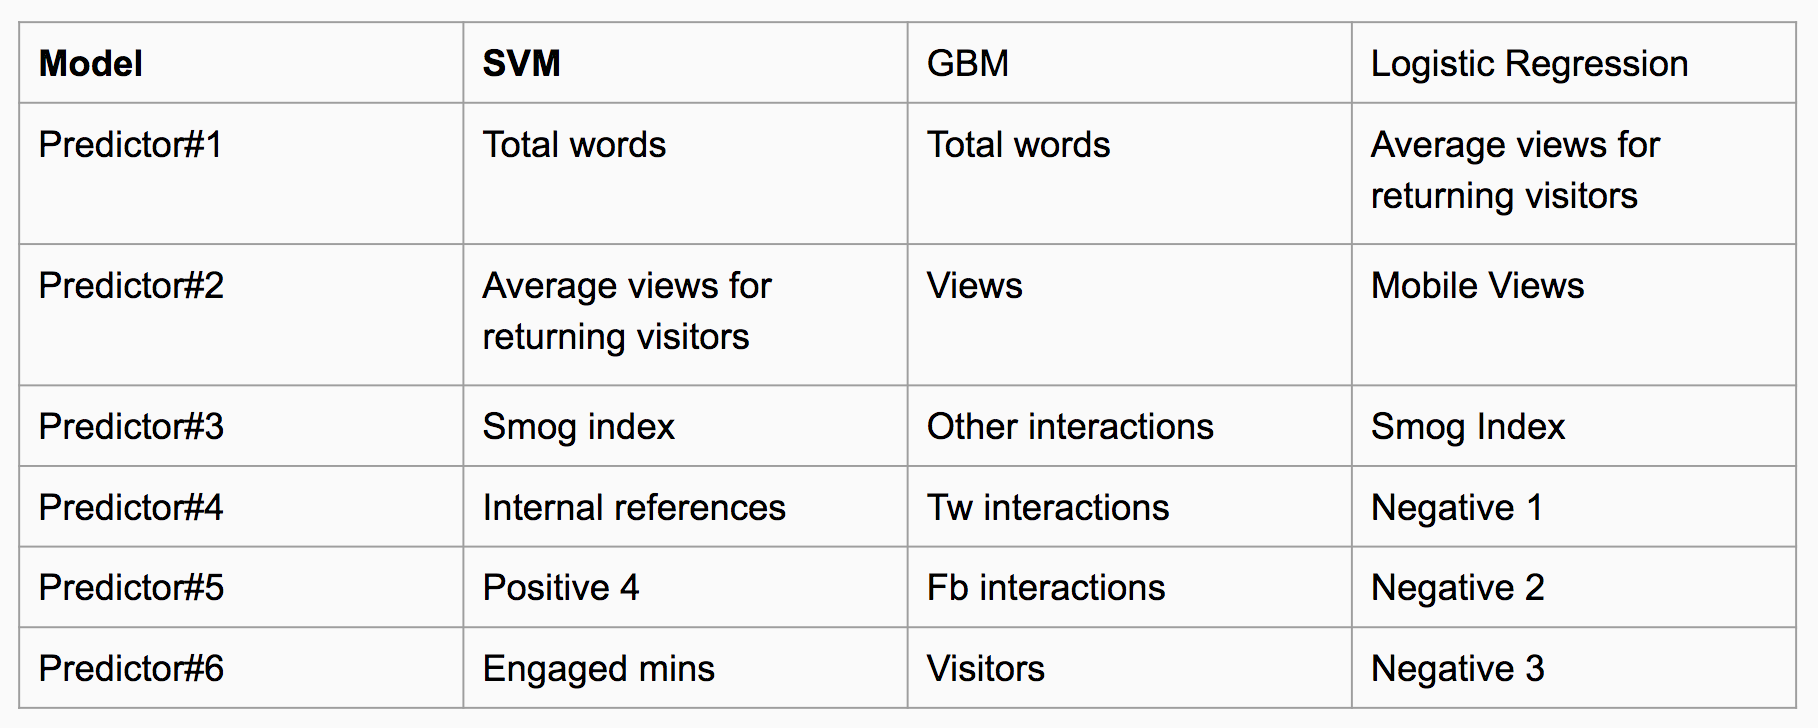
\includegraphics[width=400px]{model-comp-II} \caption{Important predictors for each of the three models in the order of importance}\label{fig:unnamed-chunk-5}
\end{figure}

Looking across our models, the table above shows how each one looks at
different variables and has different strengths. For example, the SVM
and GBM are very good at knowing which articles are socially impactful
but logistic regression is better at knowing which are not socially
impactful. We think that because the models look at different variables,
it may be reflecting on what strengths these articles have. For example,
the GBM model places an emphasis on \texttt{FB\ interaction} which none
of the other models are able to do. Therefore, if an article has an
exceptionally high or low number of Facebook interactions, its results
may be very different from the other articles.

We also looked at specificity, sensitivity, accuracy and AUROC values.

\begin{figure}
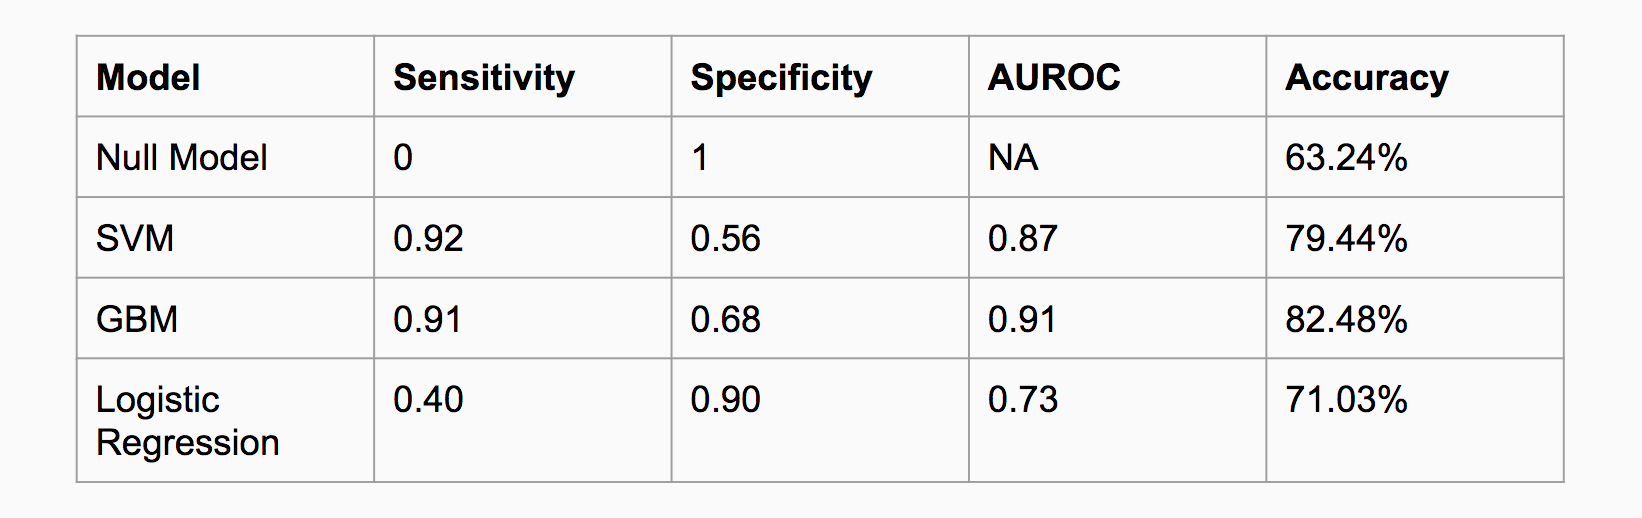
\includegraphics[width=375px]{model-comp} \caption{Table comparing performance across the four models (including the null model)}\label{fig:unnamed-chunk-6}
\end{figure}

\hypertarget{shiny-app}{%
\subsubsection{Shiny App}\label{shiny-app}}

\emph{Creation of Shiny App.} In order to display the results of our
models, a web application was created using the \texttt{Shiny} package
in R. The basic mechanism of the app starts with a user input of an
article's URL. In order for the app to correctly run, the URL must be
one of the 891 found in our SQL table. From there, multiple models
predict the article's probability of social impact. Those probabilities
are averaged. The probabilities reactively change for each article.

\emph{Method.} Three of our models are displayed on the app: the
optimized boosting model, support vector machine model, and the multiple
logistic model. Each model was saved as R data (.rda) files. These files
were loaded into an r script at the top of the app file.

An important aspect of the app's server is the SQL query. First, the app
connects to the database. Within a reactive function from the
\texttt{Shiny} package, the politics table is exported, while filtering
by the user input URL. In order to query the title, the title column is
selected from table created in the initial reactive function, and
transformed to a data frame. From there, this object is transformed into
a vector to be displayed on the app by the renderText function from the
Shiny package.

\emph{Predicting in Shiny.} Within a renderText function, the title and
URL columns from the table created in the reactive function are removed.
This new table is used within the predict function to predict the
probability of social impact from each model. These numbers are then
added to vertical lines on the distributions.

\hypertarget{interface}{%
\subsubsection{Interface}\label{interface}}

The app contains four rows. The top row contains the title of the app,
``Is this Article Socially Impactful?'' The row below contains a text
input box that prompts the user to enter a URL as well as a location for
the title of the corresponds to appear. Below this, a visualization
using ggplot2 displays the distributions of probabilities for each of
the models. Once an article is entered, vertical lines appear at the
probabilities which are predicted by each model. The fourth row displays
the probabilities from the three models as well as the average. The
probabilities are each a different color that coordinate with the
distributions and vertical lines of the visualization. A screenshot of
the app is included below in figure 7.

\begin{figure}
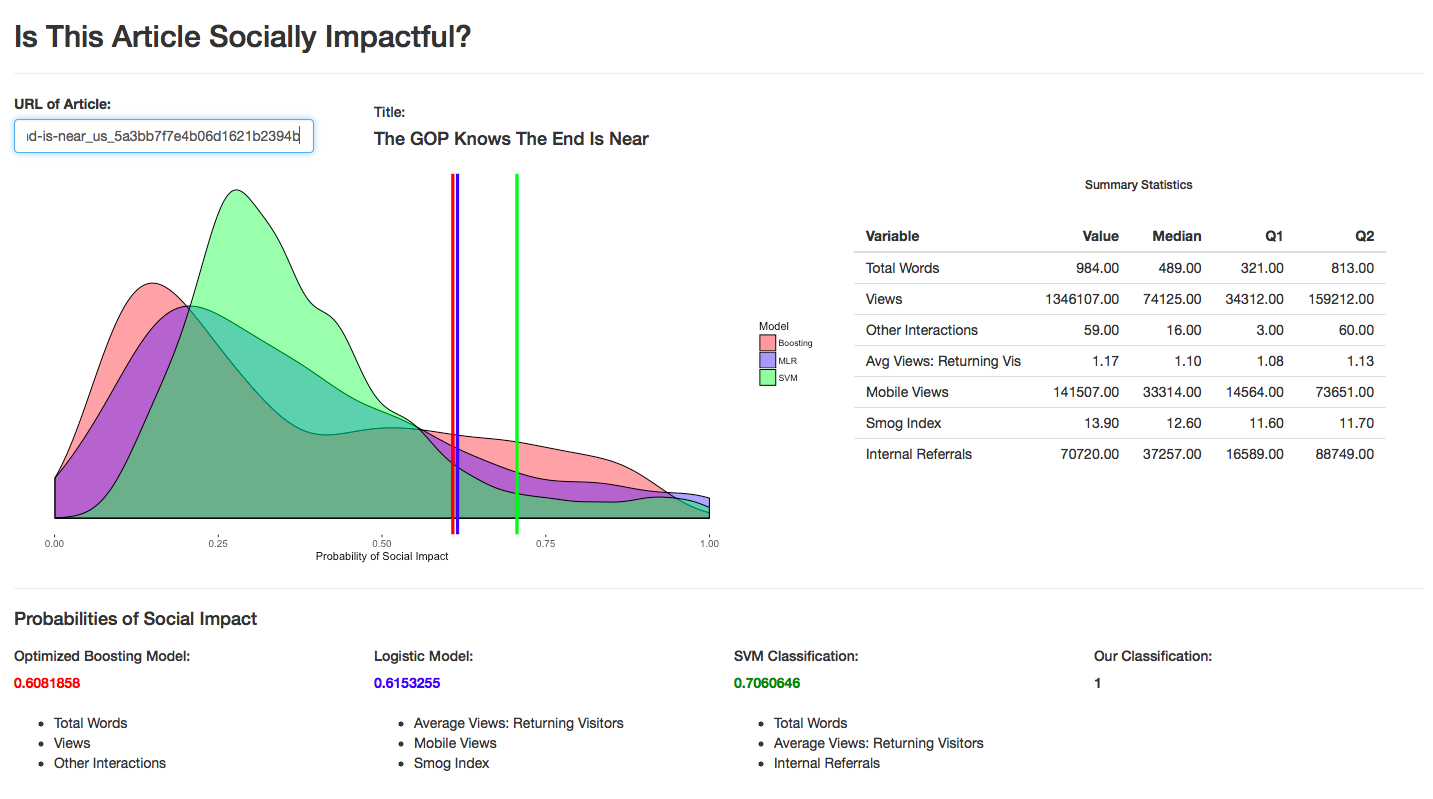
\includegraphics[width=400px,height=300px]{app} \caption{Screenshot of the app}\label{fig:unnamed-chunk-7}
\end{figure}

\hypertarget{limitations}{%
\section{Limitations}\label{limitations}}

Many of the variables in our model are connected and have high
correlations. For instance, the \texttt{Returning\_visitors} variable is
linearly dependent with average views of returning visitors and average
minutes returning visitors. The models may be using variables like these
that are connected and causing inefficiencies.

Our choice to subset our data to only politics articles may also be
considered a limitation. Instead of being able to classify any article
from our news source, it is only appropriate to use our models to
classify politics articles. Other sections may require different
variables to classify articles and our models cannot be generalized to
them.

Additionally, the pre-existing data was not randomly collected, nor did
the population of response variable random and independent. The problems
with data collection could also create biases in our models.

Despite this limitation, our group made the decision that models which
classified an article from any section would not be productive. In this
case, there would likely be a high number of both type I and II errors.
Some, like politics articles for example, may be over-classified as
socially impactful whereas others, like entertainment articles, may be
under-classified.

\hypertarget{future-work}{%
\section{Future Work}\label{future-work}}

In the future, we hope to use other data collection methods to create a
training set for our models. Possibly, adjusting our flowchart then
utilizing AMT again may be one solution. We could also attempt to find
other individuals to classify a number of articles. To solve the issues
mentioned in the limitations section, this group would need to be larger
and hopefully more representative of the entire population of those who
read these articles.

We also plan on investigating the variables in our model and make
determinations of whether they are necessary and if there are any we
could exclude to simplify our models.

We also hope to expand our interface to other sections outside of
politics too.

We would also like to explore other models.

\hypertarget{references}{%
\section*{References}\label{references}}
\addcontentsline{toc}{section}{References}

http://www2.imm.dtu.dk/pubdb/views/publication\_details.php?id=6010

\hypertarget{refs}{}
\leavevmode\hypertarget{ref-BeautifulSoup}{}%
1. Chandola V. BeautifulSoup python package. 2004.

\leavevmode\hypertarget{ref-textstat}{}%
2. Shivam Bansal CA. TextStat python package. 2011.

\leavevmode\hypertarget{ref-wikipedia_2018}{}%
3. Flesch--kincaid readability tests {[}Internet{]}. Wikipedia.
Wikimedia Foundation; 2018. Available:
\url{https://en.wikipedia.org/wiki/Flesch–Kincaid_readability_tests}

\leavevmode\hypertarget{ref-senter1967automated}{}%
4. Senter R, Smith EA. Automated readability index. CINCINNATI UNIV OH;
1967.

\leavevmode\hypertarget{ref-mclaughlin2008smog}{}%
5. McLaughlin G. SMOG: Simple measure of gobbledygook. Retreived from:
http://www harrymclaughlin com/SMOG htm. 2008;

\leavevmode\hypertarget{ref-MLbook}{}%
6. Gareth James TH Daniela Witten. A introduction to statistical
learning: With applications in r. Springer; 2013.
doi:\href{https://doi.org/10.1007/978-1-4614-7138-7}{10.1007/978-1-4614-7138-7}

\leavevmode\hypertarget{ref-Kuhn09thecaret}{}%
7. Kuhn M. The caret package. 2009.

\leavevmode\hypertarget{ref-rpart}{}%
8. Terry M. Therneau BR Beth Atkinson. Rpart: Recursive partitioning.
2011.

\leavevmode\hypertarget{ref-e1071}{}%
9. Meyer D. E1071 r package. 2017.

\nolinenumbers


\end{document}

